\documentclass[10pt,letterpaper,twocolumn]{article}
\usepackage[utf8]{inputenc}
\usepackage{amsmath}
\usepackage{amsfonts}
\usepackage{amssymb}
\usepackage{graphicx}
\usepackage{footnote}
\usepackage{float}
\usepackage{booktabs}
\usepackage{subfigure}
\usepackage{multirow}
\usepackage{tabularx} 
\usepackage{url}
\usepackage{siunitx} % Para habilitar el símbolo de ohmios (Ω)
\usepackage{tikz}
\usepackage{circuitikz}
\DeclareGraphicsExtensions{.bmp,.png,.pdf,.jpg,.eps}
\usepackage[spanish,activeacute]{babel}
%M�rgenes
\usepackage{vmargin}
\setmargins
{10mm}            % margen izquierdo
{1.5cm}           % margen superior
{190mm}           % anchura del texto
{23.42cm}         % altura del texto
{10pt}            % altura de los encabezados
{1cm}             % espacio entre el texto y los encabezados
{0pt}             % altura del pie de p�gina
{1cm}             % espacio entre el texto y el pie de p�gina


\title{\noindent\\[-4cm]\bfseries Experimento N°1}
\author{Felipe Halabi
\\\small\itshape \textit{Departamento de física, Universidad Nacional Andrés Bello, Santiago, Chile}
\\\small\itshape Física Computacional de la Materia}

\date{24 de Septiembre 2024}

\date{26 de Abril 2024}

\begin{document}
\renewcommand{\tablename}{Tabla}
\twocolumn[
\begin{@twocolumnfalse}
\maketitle
\begin{abstract}
El objetivo de este experimento es estudiar la interacción de los átomos para una celda del gas noble Xenon, en el cual se analizara el comportamiento de la temperatura, energía cinética, energía potencial y el número de coordinación a través de simulaciones computacionales en el software Las Palmeras Molecular Dynamics (lpmd).

\vspace{5mm}

\end{abstract}
\end{@twocolumnfalse}
\noindent\
]
\section*{Introducción}
El Xenón (Xe) es un elemento químico perteneciente al grupo de los gases nobles, con número atómico 54. Es un gas incoloro, inodoro, y no reactivo en condiciones normales, conocido por su estabilidad química y su baja reactividad debido a su configuración electrónica completa. A diferencia de otros gases nobles más ligeros como el helio, el xenón puede formar algunos compuestos en condiciones extremas debido a su mayor número de electrones y su capacidad para expandir su capa de valencia.

El Xenón cristaliza en estructuras cúbicas centradas en las caras (FCC) a bajas temperaturas, lo que significa que en estado sólido sus átomos están dispuestos en una red en la que cada átomo tiene 12 vecinos más cercanos, en una disposición de alta simetría y densidad empacada.

% \begin{figure}[h]
%     \centering
%     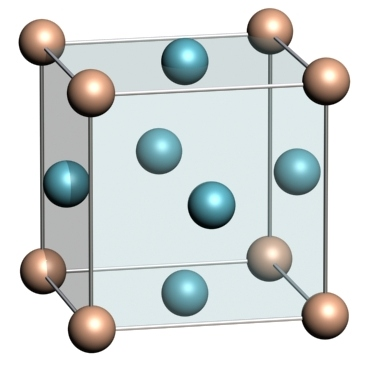
\includegraphics[width=0.3\linewidth]{FCCStructure.jpg}
%     \caption{Caption}
%     \label{fig:enter-label}
% \end{figure}

Para la construcción de la estructura cristalina del Xenón (Xe), también es necesario considerar 3 aristas y 3 ángulos que permiten formar su modelo estructural. En el caso del xenón en estado sólido, cristaliza en una estructura cúbica centrada en las caras (FCC), que se caracteriza por tener átomos en cada vértice del cubo y en el centro de cada una de sus caras.

Las aristas a, b, y c corresponden a los lados del cubo que forman la red cúbica de alta simetría. En esta estructura, todos los ángulos \si{\alpha}, \si{\beta} y \si{\gamma} son de 90°, ya que la disposición cúbica implica ángulos rectos entre los ejes del cubo.

El radio atómico del xenón sólido en la red FCC es de aproximadamente 4.34 Å, lo que proporciona la distancia entre los centros de los átomos adyacentes. Esta disposición geométrica de alta densidad empaqueta los átomos de manera eficiente en tres dimensiones.

Una de las propiedades distintivas del xenón es su relativamente alto punto de ebullición comparado con otros gases nobles más ligeros. El xenón hierve a una temperatura de 165.03 K (-108.12 °C).

Al ser un elemento en el cual se encuentra en temperaturas bajo el umbral de los $0^{\circ}C$, para lograr llegar al estado de solidificación es necesario que este gas se encuentre a una temperatura de $4K$, esta solidificación no se encuentra en situaciones comunes por lo
que esta fase sería rara de formularse al no ser una estructura cristalina.
Al existir una cantidad de átomos que interactúan entre ellos, es esencial hablar del potencial propuesto por Lennard Jones en 1924[3]. Este potencial describe la energía potencial del estado ligado de una molécula diatómica para una configuración electrónica dada, esta interacción viene dada mediante la siguiente ecuación:

\begin{equation}
    U(r)=4\epsilon[(\dfrac{\sigma}{r})^{12} - (\dfrac{\sigma}{r})^{6}]
\end{equation}

Donde $U(r)$ es la energía potencial intermolecular en función de la distancia de separación entre un par de moléculas, $\epsilon$ es la profundidad del pozo potencial en Joule y $\sigma$ es el valor finito de la distancia en Ángstroms $\r{A}$ en el cual el potencial entre partículas se vuelve cero.
Gracias a un artículo publicado el año 2013 por Seung-Kyo Oh, es posible
obtener los parámetros del potencial de Lennard-Jones para los gases nobles
mediante la siguiente tabla.

\begin{table}[h] % La 'h' sugiere a LaTeX que coloque la tabla aquí mismo
\centering % Centra horizontalmente la tabla
\begin{tabular}{cccc}
\toprule
Gropu & $\sigma$\slash$\r{A}$ & $($\epsilon$ \slash $\k_{B})$ \\
\midrule 
1  & 1.43 \\
2  & 1.33 \\
3  & 1.45 \\
4  & 1.50 \\

\bottomrule
\end{tabular}
\caption{Periodos de oscilación medidos}
\label{tab:periodos_oscilacion}
\end{table}

\section*{Información Relevante}

Profesor : Carlos Curín Retamal \\

Nombre : José Luis Soto Pezoa\\
correo : j.sotopezoa@uandresbello.edu

Nombre : Felipe Halabi Alcayaga\\
correo : f.halabialcayaga@uandresbello.edu

\end{document}

